\begin{definition}
    Giả sử hai toạ độ $x$, $y$ trên mặt phẳng toạ độ lần lượt là các hàm của một biến thứ ba, $t$ (gọi là \emph{tham số}) được biểu diễn qua các phương trình:
     \begin{equation*}   x=f(t),\ y=g(t),
\end{equation*}
    gọi là các \emph{phương trình tham số}. Mỗi một giá trị của $t$ xác định một điểm $(x;y)$. Khi tham số thay đổi, điểm $(x;y)$ thay đổi và vẽ ra một đường cong trên mặt phẳng toạ độ gọi là \emph{đường cong tham số}.
\end{definition}

% Add this line to your preamble (at the top of your .tex file, before \begin{document})

\newpage

\begin{figure}[!htbp]
    \centering
    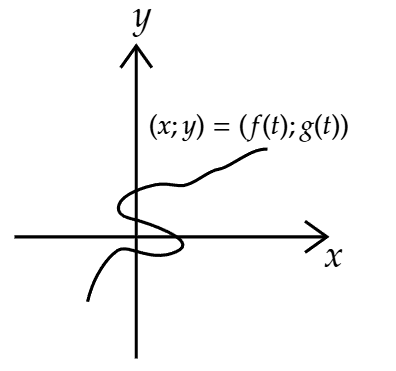
\includegraphics[width=0.3\textwidth, height=0.2\textheight]{Tuan1/ảnh/parameter.png}
    \caption{Đường cong tham số}
    \label{fig:phuongtrinhthamso}   
\end{figure}    
\vspace{-0.5em}
Về tổng quát, đường cong với phương trình tham số $x=f(t), y=g(t), a\leq t\leq b$ có điểm đầu $(f(a),g(a))$ và điểm cuối $(f(b),g(b))$. \newline Sau đây là một số ví dụ cụ thể:
\vspace{-1.75em}
\begin{figure}[H]
    \centering
    \begin{subfigure}{0.45\textwidth}
        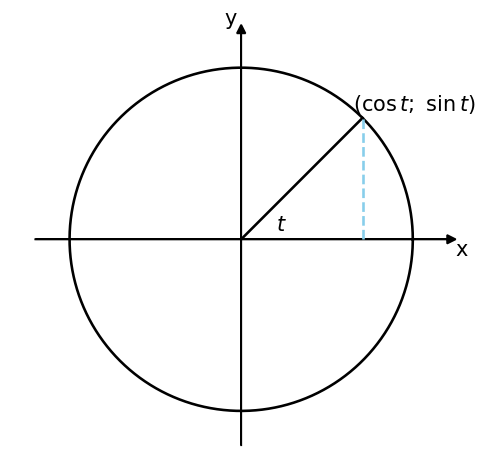
\includegraphics[width=\linewidth]{Tuan1/ảnh/duongtronthamso.png}
        \caption{ Đường tròn đơn vị \newline\hspace*{1em} \(x=\cos t,\quad y=\sin t\)\newline \hspace*{1em} \(0\leq t\leq 2\pi\)}
    \end{subfigure}
    \hspace{\fill}
    \begin{subfigure}{0.45\textwidth}
        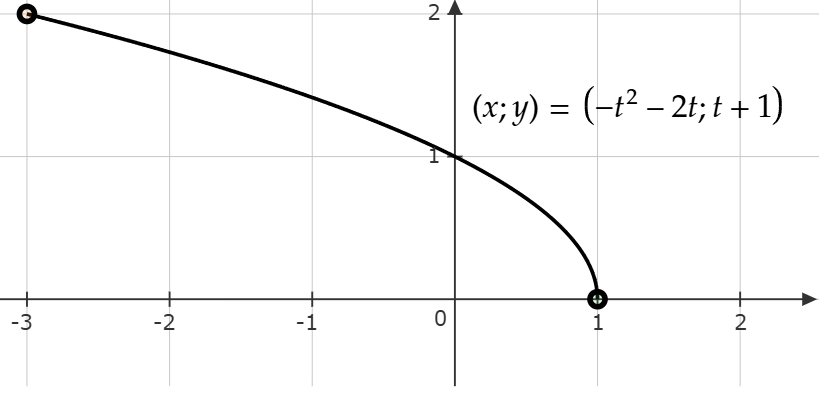
\includegraphics[width=\linewidth]{Tuan1/ảnh/parabolngang.png}
        \caption{Parabol nằm ngang \newline\hspace*{1em}\(x=t^2 -1,\quad y=t\)\newline\hspace*{1em} \(-1\leq t\leq 1\)}
    \end{subfigure}
    \caption{}
\end{figure}

<<<<<<< HEAD
\begin{figure}[H]
    \centering
    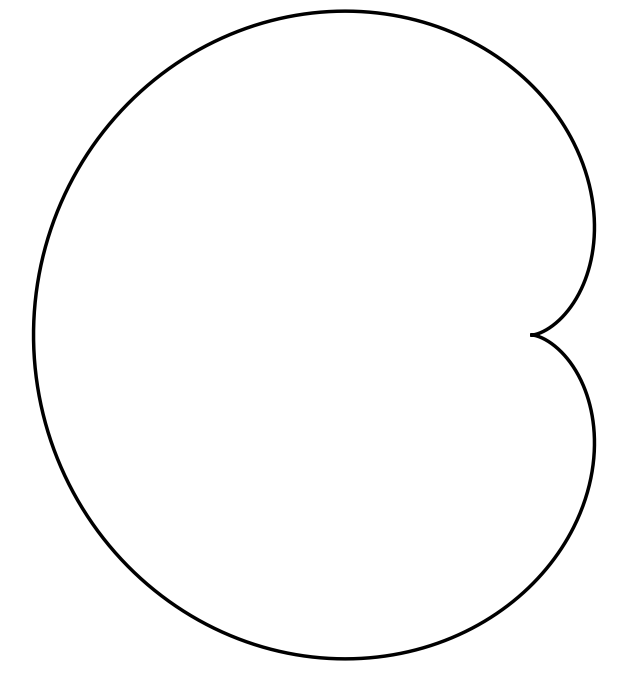
\includegraphics[width=0.3\linewidth]{Tuan1/ảnh/cardioid.png}
    \caption{Đường Cardioid\newline \hspace*{1em} $x = 2\cos t - \cos 2t,\quad y = 2\sin t - \sin 2t$}
\end{figure}

\begin{figure}[H]
    \centering
    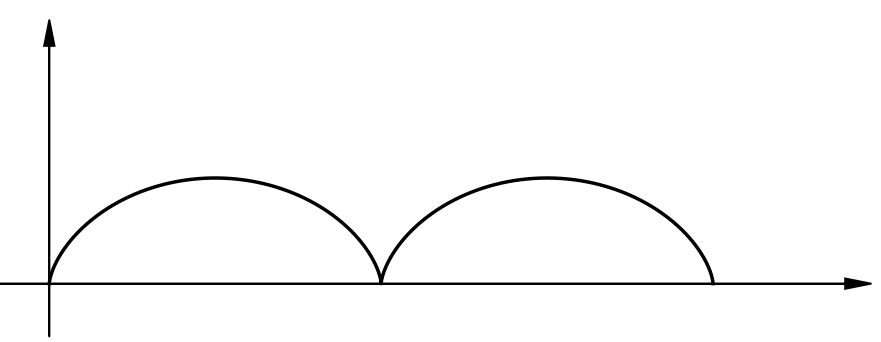
\includegraphics[width=0.5\linewidth]{Tuan1/ảnh/cycloid.png}
    \caption{Đường Cycloid\newline \hspace*{1em} $x=t-\sin t,\quad y=1-\cos t\quad (0\leq t\leq 4\pi)$}
\end{figure}

Thông thường khi tiếp cận một bài toán chuyển động, tham số thường xuất hiện một cách tự nhiên qua các đại lượng vật lý mà điển hình là thời gian.\newline
Xem xét một điểm chuyển động trên mặt phẳng toạ độ,  hai toạ độ sẽ có dạng $x=x(t)$ và $y=y(t)$. Đây được gọi là các phương trình chuyển động, nếu biết chúng và điều kiện ban đầu sẽ có thể biết được các thông số động học của nó ở mọi thời điểm. Các thông số động học được đề cập ở đây là \emph{vị trí}, \emph{vận tốc},... , trong đó ta định nghĩa:
\begin{itemize}
    \item Vị trí của điểm $t=\tau$ được xác định bởi cặp số $(x(\tau),y(\tau))$.
    \item Vận tốc của điểm tại thời điểm $t=\tau$ được xác định bởi cặp số $(x'(\tau),y'(\tau))$.
\end{itemize}
=======
    Thông thường khi tiếp cận các bài toán về chuyển động, tham số $t$ thường xuất hiện một cách tự nhiên thông qua các đại lượng. Trong đó điển hình là thời gian.\newline
    Xét một điểm chuyển động trên mặt phẳng toạ độ, \emph{hệ phương trình chuyển động} của nó có dạng: \newline
    % \begin{cases}
    %     \item $x=x(t)$,
    %     \item $y=y(t)$.
    % \end{cases}
    Hệ phương trình chuyển động này mô tả sự phụ thuộc của các toạ độ của điểm theo thời gian và đồng thời bao hàm cả quỹ đạo của nó nếu biết các điều kiện đầu và cuối.
    \begin{definition}
        \begin{equation}
            v_{x} (v_y)=\frac{dx}{dt}\left(\frac{dy}{dt}\right)
        \end{equation}
    được gọi là thành phần \emph{vận tốc} của điểm đó trên trục $Ox(Oy)$.
    \end{definition}
    \begin{definition}
        \begin{equation}
            a_{x}(a_y)=\frac{dv_x}{dt}\left(\frac{dv_y}{dt}\right)=\frac{d^2x}{dt^2}\left(\frac{d^2y}{dt^2}\right)
        \end{equation}
    được gọi là thành phần \emph{gia tốc} của điểm đó trên trục $Ox(Oy)$.
    \end{definition}
    
>>>>>>> 034e26e813f325d967f66d2871efe4ac7d54c9a0
